% =============================================================================
% Janus Lab -- Lecture 02: Hardware and CPU Verification
% Covers: simulation, testbenches, waveforms, assertions, coverage, formal,
%         CPU-specific verification, and IIC-OSIC-TOOLS lab workflow
% Compile with: pdflatex 02_cpu_verification.tex  (twice for ToC/overlays)
% =============================================================================
\documentclass[aspectratio=169,10pt]{beamer}

% -- Theme --------------------------------------------------------------------
\usetheme{Madrid}
\usecolortheme{beaver}
\setbeamertemplate{navigation symbols}{}
\setbeamertemplate{footline}[frame number]
\setbeamerfont{frametitle}{size=\normalsize,series=\bfseries}

% -- Packages -----------------------------------------------------------------
\usepackage{booktabs}
\usepackage{array}
\usepackage{colortbl}
\usepackage{listings}
\usepackage{tikz}
\usepackage{pgf}
\usepackage{xcolor}
\usepackage{fontawesome5}
\usepackage{amsmath}
\usepackage{graphicx}
\usepackage{microtype}

\usetikzlibrary{arrows.meta, shapes.geometric, positioning, fit, backgrounds, calc}

% -- Listing styles -----------------------------------------------------------
\lstdefinelanguage{Verilog}{
  morekeywords={module,endmodule,input,output,wire,reg,logic,always,posedge,
    negedge,begin,end,if,else,case,endcase,assign,parameter,localparam,
    initial,default,integer,for,generate,endgenerate,function,endfunction,
    task,endtask,property,endproperty,assert,cover,assume},
  sensitive=true,
  morecomment=[l]{//},
  morecomment=[s]{/*}{*/},
  morestring=[b]"
}
\lstdefinelanguage{Shell}{
  morekeywords={cd,make,docker,podman,git,verilator,iverilog,vvp,gtkwave,
    yosys,sby,python3,riscv64-unknown-elf-as,riscv64-unknown-elf-ld,
    riscv64-unknown-elf-objcopy,spike},
  sensitive=true,
  morecomment=[l]{\#},
  morestring=[b]"
}
\lstset{
  language=Verilog,
  basicstyle=\ttfamily\scriptsize,
  keywordstyle=\color{blue!70!black}\bfseries,
  commentstyle=\color{gray}\itshape,
  stringstyle=\color{red!70!black},
  backgroundcolor=\color{black!4},
  frame=single,
  framerule=0.4pt,
  xleftmargin=6pt,
  xrightmargin=6pt,
  breaklines=true,
  tabsize=4,
  showstringspaces=false,
}

% -- Colour palette -----------------------------------------------------------
\definecolor{janusblue}{RGB}{25,70,140}
\definecolor{janusred}{RGB}{180,30,30}
\definecolor{janusgray}{RGB}{90,90,90}
\definecolor{verifygreen}{RGB}{42,130,70}
\definecolor{warnorange}{RGB}{225,130,35}
\definecolor{bugred}{RGB}{185,45,45}
\definecolor{deepviolet}{RGB}{95,75,160}
\definecolor{stageIF}{RGB}{198,224,180}
\definecolor{stageID}{RGB}{180,198,231}
\definecolor{stageEX}{RGB}{255,217,102}
\definecolor{stageMEM}{RGB}{248,203,173}
\definecolor{stageWB}{RGB}{217,173,248}
\definecolor{pipeboxbg}{RGB}{245,245,245}

% -- Title info ---------------------------------------------------------------
\title[Janus Lab -- CPU Verification]{Janus Lab: Verifying a Tiny RISC-V CPU}
\subtitle{Lecture 02 --- Hardware Verification, CPU Verification, and Open-Source Tools}
\author{Janus Lab}
\date{\today}
\institute{CPU Design and Implementation}

% =============================================================================
\begin{document}
% =============================================================================

% -- Title frame ---------------------------------------------------------------
\begin{frame}
  \titlepage
\end{frame}

% -- Outline ------------------------------------------------------------------
\begin{frame}{Outline}
  \tableofcontents
\end{frame}

% =============================================================================
\section{Verification Mindset}
% =============================================================================

\begin{frame}{Why This Lecture Comes After Your First CPU}
  \begin{columns}[T]
    \begin{column}{0.52\textwidth}
      In Lecture 01 and Lab 01, you built a working RV32I CPU demo.

      \vspace{0.8em}
      Now the question changes from:
      \begin{center}
        \large\textbf{``Can it run my demo?''}
      \end{center}
      to:
      \begin{center}
        \large\textbf{``How do I know it is actually correct?''}
      \end{center}

      \vspace{0.8em}
      A CPU can pass one program while still being wrong for:
      \begin{itemize}
        \item corner-case immediates, shifts, signed comparisons, and alignment
        \item pipeline hazards: stale operands, missing stalls, wrong flushes
        \item reset behavior and unknown values
        \item rare instruction sequences nobody tried manually
      \end{itemize}
    \end{column}
    \begin{column}{0.42\textwidth}
      \begin{block}{Lecture 02 Goal}
        Learn the verification vocabulary, tools, and workflow needed to test your own CPU inside the IIC-OSIC-TOOLS container.
      \end{block}

      \vspace{0.6em}
      \begin{exampleblock}{End of Lecture Capability}
        You should be able to:
        \begin{itemize}\small
          \item write a simple self-checking testbench
          \item run RTL simulation
          \item inspect a waveform
          \item create directed CPU tests
          \item explain what coverage and assertions are
          \item debug a failing pipeline test systematically
        \end{itemize}
      \end{exampleblock}
    \end{column}
  \end{columns}
\end{frame}

\begin{frame}{What Does ``Verification'' Mean?}
  \begin{columns}[T]
    \begin{column}{0.48\textwidth}
      \textbf{Design} is the act of building the hardware:
      \begin{itemize}
        \item RTL modules such as \texttt{alu}, \texttt{reg\_file}, \texttt{cpu}
        \item datapath wires, control logic, pipeline registers
        \item memory interfaces and reset behavior
      \end{itemize}

      \vspace{0.8em}
      \textbf{Verification} is the act of collecting evidence that the design satisfies its specification:
      \begin{itemize}
        \item ``Does \texttt{ADD} compute modulo-32-bit addition?''
        \item ``Does \texttt{x0} always read as zero?''
        \item ``Does a taken branch flush the wrong-path instructions?''
        \item ``Can a load-use dependency ever consume stale data?''
      \end{itemize}
    \end{column}
    \begin{column}{0.48\textwidth}
      \begin{block}{A Useful Formula}
        \centering
        \Large
        Spec + Tests + Checks + Debug = Confidence
      \end{block}

      \vspace{0.8em}
      \begin{alertblock}{Important Limitation}
        Verification rarely proves that a complex CPU is perfect. Most verification work is about reducing risk by attacking the design from many angles.
      \end{alertblock}

      \vspace{0.8em}
      \small
      In this lab, ``correct'' means the RTL behavior matches the Janus Lab CPU specification and the RV32I architectural rules for the implemented instruction subset.
    \end{column}
  \end{columns}
\end{frame}

\begin{frame}{Hardware Bugs Are Different from Software Bugs}
  \begin{columns}[T]
    \begin{column}{0.47\textwidth}
      \textbf{Software mental model}
      \begin{itemize}
        \item one instruction stream executes in sequence
        \item variables update when the program reaches that line
        \item a debugger can stop at a line of code
        \item tests call functions and check return values
      \end{itemize}

      \vspace{0.7em}
      \begin{block}{Software example}
        \texttt{result = add(a, b)} returns once; then the next statement runs.
      \end{block}
    \end{column}
    \begin{column}{0.47\textwidth}
      \textbf{Hardware mental model}
      \begin{itemize}
        \item many signals change at the same time
        \item combinational logic reacts continuously
        \item registers update together on clock edges
        \item a waveform shows signal history over simulated time
      \end{itemize}

      \vspace{0.7em}
      \begin{block}{Hardware example}
        At a clock edge, \texttt{pc}, \texttt{IF/ID}, \texttt{ID/EX}, \texttt{EX/MEM}, and \texttt{MEM/WB} may all update together.
      \end{block}
    \end{column}
  \end{columns}

  \vspace{0.8em}
  \begin{center}
    \small\textbf{CPU verification is mostly about time:} which value is visible in which pipeline stage on which cycle?
  \end{center}
\end{frame}

\begin{frame}{Verification Vocabulary}
  \renewcommand{\arraystretch}{1.25}
  \small
  \begin{tabular}{>{\bfseries\ttfamily}l p{10.5cm}}
    \toprule
    Term & Meaning \\
    \midrule
    RTL & Register-Transfer Level. Verilog/SystemVerilog code describing registers and combinational logic. \\
    DUT & Design Under Test. The hardware block being verified, such as \texttt{alu} or \texttt{cpu}. \\
    UUT & Unit Under Test. Same idea as DUT; often used for small modules. \\
    Testbench & Simulation-only code that drives inputs, clocks the DUT, observes outputs, and decides pass/fail. \\
    Stimulus & Input activity given to the DUT: reset pulses, instructions, memory contents, random values. \\
    Checker & Code that detects incorrect behavior. Examples: \texttt{if} checks, assertions, scoreboards. \\
    Oracle & Trusted source of expected behavior, such as hand-computed results or the Spike RISC-V ISA simulator. \\
    Waveform & Time plot of signals dumped to VCD/FST and opened in GTKWave or another viewer. \\
    Coverage & Measurement of what behavior was exercised by tests: code lines, branches, instructions, hazards. \\
    Regression & Re-running many tests automatically after every change to catch newly introduced bugs. \\
    \bottomrule
  \end{tabular}
\end{frame}

\begin{frame}{The Verification Loop}
  \begin{center}
  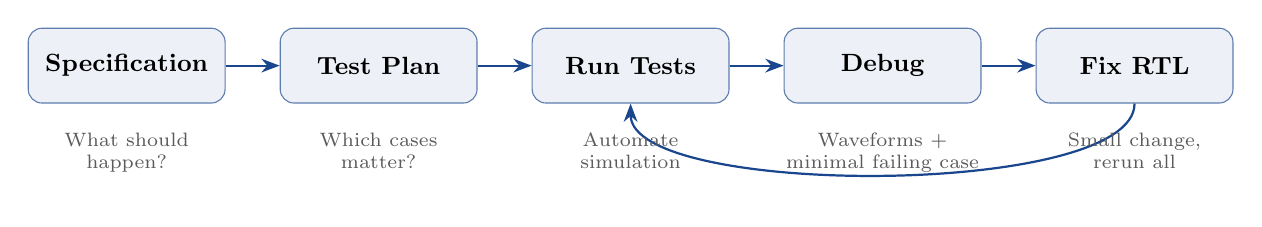
\begin{tikzpicture}[
    box/.style={draw=janusblue!70, fill=janusblue!8, rounded corners=5pt,
                minimum width=2.5cm, minimum height=0.95cm, align=center,
                font=\small\bfseries},
    note/.style={font=\scriptsize, text=janusgray, align=center},
    arr/.style={-Stealth, thick, janusblue}
  ]
    \node[box] (spec) at (0,0) {Specification};
    \node[box] (plan) at (3.2,0) {Test Plan};
    \node[box] (run)  at (6.4,0) {Run Tests};
    \node[box] (fail) at (9.6,0) {Debug};
    \node[box] (fix)  at (12.8,0) {Fix RTL};

    \draw[arr] (spec) -- (plan);
    \draw[arr] (plan) -- (run);
    \draw[arr] (run) -- (fail);
    \draw[arr] (fail) -- (fix);
    \draw[arr] (fix.south) .. controls +(0,-1.2) and +(0,-1.2) .. (run.south);

    \node[note, below=0.25cm of spec] {What should\\happen?};
    \node[note, below=0.25cm of plan] {Which cases\\matter?};
    \node[note, below=0.25cm of run] {Automate\\simulation};
    \node[note, below=0.25cm of fail] {Waveforms +\\minimal failing case};
    \node[note, below=0.25cm of fix] {Small change,\\rerun all};
  \end{tikzpicture}
  \end{center}

  \vspace{1em}
  \begin{exampleblock}{Practical Rule}
    Never debug only by staring at RTL. First create a failing test, then use the waveform to locate the first cycle where actual behavior diverges from expected behavior.
  \end{exampleblock}
\end{frame}

% =============================================================================
\section{Simulation Basics}
% =============================================================================

\begin{frame}{How Hardware Simulation Works}
  \begin{columns}[T]
    \begin{column}{0.50\textwidth}
      An RTL simulator evaluates your Verilog model over \textbf{simulated time}.

      \vspace{0.7em}
      \textbf{Two kinds of logic}
      \begin{itemize}
        \item \textbf{Combinational logic:} output changes when input changes
        \item \textbf{Sequential logic:} register output changes on a clock edge
      \end{itemize}

      \vspace{0.7em}
      \textbf{Testbench responsibilities}
      \begin{itemize}
        \item create the clock and reset
        \item load memories or drive input pins
        \item choose when simulation stops
        \item print pass/fail
        \item dump waveforms for debugging
      \end{itemize}
    \end{column}
    \begin{column}{0.46\textwidth}
      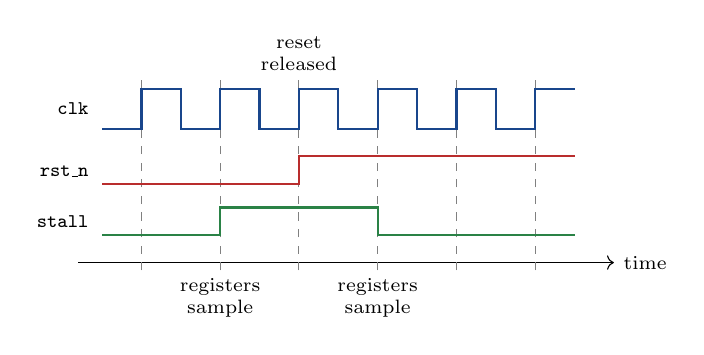
\begin{tikzpicture}[
        sig/.style={thick},
        edge/.style={dashed, gray},
        lab/.style={font=\scriptsize}
      ]
        \draw[->] (0,0) -- (6.8,0) node[right, lab] {time};
        \foreach \x in {0.8,1.8,2.8,3.8,4.8,5.8} {
          \draw[edge] (\x,-0.1) -- (\x,2.4);
        }
        \draw[sig, janusblue] (0.3,1.7) -- (0.8,1.7) -- (0.8,2.2) -- (1.3,2.2)
          -- (1.3,1.7) -- (1.8,1.7) -- (1.8,2.2) -- (2.3,2.2)
          -- (2.3,1.7) -- (2.8,1.7) -- (2.8,2.2) -- (3.3,2.2)
          -- (3.3,1.7) -- (3.8,1.7) -- (3.8,2.2) -- (4.3,2.2)
          -- (4.3,1.7) -- (4.8,1.7) -- (4.8,2.2) -- (5.3,2.2)
          -- (5.3,1.7) -- (5.8,1.7) -- (5.8,2.2) -- (6.3,2.2);
        \node[lab, left] at (0.25,1.95) {\texttt{clk}};

        \draw[sig, bugred] (0.3,1.0) -- (2.8,1.0) -- (2.8,1.35) -- (6.3,1.35);
        \node[lab, left] at (0.25,1.16) {\texttt{rst\_n}};

        \draw[sig, verifygreen] (0.3,0.35) -- (1.8,0.35) -- (1.8,0.7)
          -- (3.8,0.7) -- (3.8,0.35) -- (6.3,0.35);
        \node[lab, left] at (0.25,0.52) {\texttt{stall}};

        \node[lab, align=center] at (2.8,2.65) {reset\\released};
        \node[lab, align=center] at (1.8,-0.45) {registers\\sample};
        \node[lab, align=center] at (3.8,-0.45) {registers\\sample};
      \end{tikzpicture}

      \vspace{0.6em}
      \begin{block}{Clock Edge}
        In this lab, state changes on \texttt{posedge clk}. Reset is active-low: \texttt{rst\_n = 0} means reset is asserted.
      \end{block}
    \end{column}
  \end{columns}
\end{frame}

\begin{frame}[fragile]{The Smallest Useful Testbench}
  \begin{columns}[T]
    \begin{column}{0.49\textwidth}
      A testbench is not synthesized into hardware. It is a simulation program for controlling and checking the DUT.

      \vspace{0.6em}
      \textbf{This example tests an ALU add operation:}
      \begin{itemize}
        \item instantiate the DUT
        \item drive inputs
        \item wait one time step for combinational logic
        \item compare actual output with expected output
        \item call \texttt{\$finish}
      \end{itemize}
    \end{column}
    \begin{column}{0.47\textwidth}
\begin{lstlisting}
module tb_alu;
  reg  [31:0] a, b;
  reg  [3:0]  alu_ctrl;
  wire [31:0] result;
  wire        zero;

  alu dut (
    .a(a), .b(b),
    .alu_ctrl(alu_ctrl),
    .result(result),
    .zero(zero)
  );

  initial begin
    a = 32'd7;
    b = 32'd5;
    alu_ctrl = 4'd0; // ADD
    #1;
    if (result !== 32'd12) begin
      $display("FAIL: got %h", result);
      $finish;
    end
    $display("PASS");
    $finish;
  end
endmodule
\end{lstlisting}
    \end{column}
  \end{columns}
\end{frame}

\begin{frame}[fragile]{Clock and Reset in the Janus Testbench}
  \begin{columns}[T]
    \begin{column}{0.49\textwidth}
      The lab testbench \texttt{cpu/tb\_top.v} creates a 100 MHz simulation clock:

      \vspace{0.7em}
      \begin{itemize}
        \item \texttt{CLK\_PERIOD = 10} ns
        \item \texttt{clk} toggles every 5 ns
        \item reset is held low for four rising edges
        \item reset release is aligned to a negative edge, so the next positive edge sees stable \texttt{rst\_n = 1}
      \end{itemize}

      \vspace{0.7em}
      \begin{alertblock}{Reset Bugs Are Common}
        If the PC or pipeline registers are not reset, the CPU may fetch from an unknown address and the whole waveform becomes meaningless.
      \end{alertblock}
    \end{column}
    \begin{column}{0.47\textwidth}
\begin{lstlisting}
reg clk;
reg rst_n;

localparam CLK_PERIOD = 10; // ns

initial clk = 1'b0;
always #(CLK_PERIOD / 2) clk = ~clk;

initial begin
  rst_n = 1'b0;
  repeat (4) @(posedge clk);
  @(negedge clk);
  rst_n = 1'b1;
end
\end{lstlisting}
      \vspace{0.4em}
      \small
      The \texttt{always} block repeats forever. The \texttt{initial} block runs once at time zero.
    \end{column}
  \end{columns}
\end{frame}

\begin{frame}{Four-State Logic: \texttt{0}, \texttt{1}, \texttt{X}, and \texttt{Z}}
  \begin{columns}[T]
    \begin{column}{0.50\textwidth}
      Verilog simulation usually uses \textbf{four-state logic}:
      \begin{itemize}
        \item \texttt{0}: known logic low
        \item \texttt{1}: known logic high
        \item \texttt{X}: unknown value
        \item \texttt{Z}: high impedance, usually an undriven tri-state wire
      \end{itemize}

      \vspace{0.8em}
      \textbf{Why \texttt{X} matters}
      \begin{itemize}
        \item uninitialized registers start as \texttt{X}
        \item missing \texttt{case} defaults can create \texttt{X}
        \item comparing with \texttt{==} can hide unknowns
        \item comparing with \texttt{===} or \texttt{!==} catches exact four-state values
      \end{itemize}
    \end{column}
    \begin{column}{0.46\textwidth}
      \begin{block}{Bad Check}
        \texttt{if (result != expected)} may not fail when \texttt{result} contains unknown bits.
      \end{block}

      \vspace{0.7em}
      \begin{exampleblock}{Better Check in Testbenches}
        \texttt{if (result !== expected)} uses case inequality and detects \texttt{X}/\texttt{Z} mismatches.
      \end{exampleblock}

      \vspace{0.7em}
      \begin{alertblock}{Design Rule}
        Every sequential register that affects architectural behavior should have a reset value or be deliberately initialized before use.
      \end{alertblock}
    \end{column}
  \end{columns}
\end{frame}

\begin{frame}[fragile]{Observability: \texttt{\$display}, VCD, and GTKWave}
  \begin{columns}[T]
    \begin{column}{0.50\textwidth}
      A simulator can tell you pass/fail, but a waveform explains \textbf{why}.

      \vspace{0.7em}
      \textbf{Common tools}
      \begin{itemize}
        \item \texttt{\$display}: print text during simulation
        \item \texttt{\$dumpfile}: choose waveform output filename
        \item \texttt{\$dumpvars}: choose which signals are recorded
        \item VCD: Value Change Dump, a standard text waveform format
        \item GTKWave: GUI waveform viewer for VCD/FST files
      \end{itemize}
    \end{column}
    \begin{column}{0.46\textwidth}
\begin{lstlisting}
initial begin
  $dumpfile("dump.vcd");
  $dumpvars(0, tb_top);
end

always @(posedge clk) begin
  $display("cycle=%0d pc=%08h",
           cycle_count,
           u_cpu.u_pc_reg.pc);
end
\end{lstlisting}

      \vspace{0.4em}
      \begin{block}{Waveform Scope}
        \texttt{\$dumpvars(0, tb\_top)} dumps everything below \texttt{tb\_top}. This is convenient for debugging but can create large files.
      \end{block}
    \end{column}
  \end{columns}
\end{frame}

\begin{frame}{Open-Source Tool Map}
  \begin{center}
  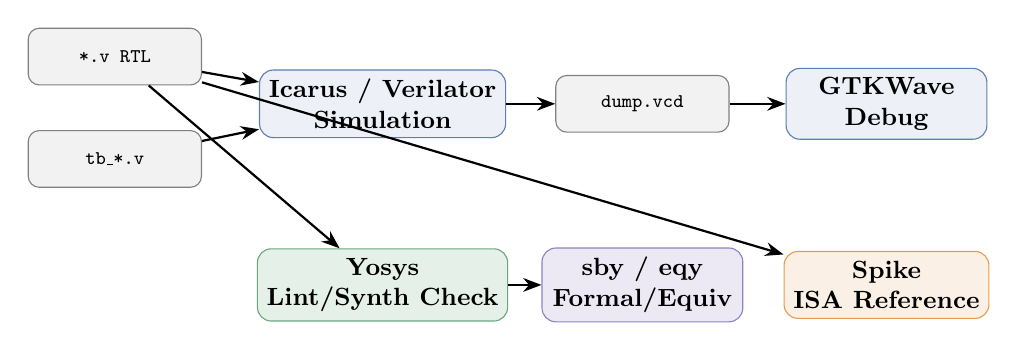
\begin{tikzpicture}[
    tool/.style={draw=janusblue!70, fill=janusblue!8, rounded corners=5pt,
                 minimum width=2.55cm, minimum height=0.85cm,
                 align=center, font=\small\bfseries},
    file/.style={draw=black!50, fill=black!5, rounded corners=4pt,
                 minimum width=2.2cm, minimum height=0.72cm,
                 align=center, font=\scriptsize\ttfamily},
    arr/.style={-Stealth, thick}
  ]
    \node[file] (rtl) at (0,1.6) {*.v RTL};
    \node[file] (tb)  at (0,0.3) {tb\_*.v};
    \node[tool] (sim) at (3.4,1.0) {Icarus / Verilator\\Simulation};
    \node[file] (vcd) at (6.7,1.0) {dump.vcd};
    \node[tool] (wave) at (9.8,1.0) {GTKWave\\Debug};

    \node[tool, fill=verifygreen!12, draw=verifygreen!70] (yosys) at (3.4,-1.3) {Yosys\\Lint/Synth Check};
    \node[tool, fill=deepviolet!12, draw=deepviolet!70] (formal) at (6.7,-1.3) {sby / eqy\\Formal/Equiv};
    \node[tool, fill=warnorange!12, draw=warnorange!80] (iss) at (9.8,-1.3) {Spike\\ISA Reference};

    \draw[arr] (rtl) -- (sim);
    \draw[arr] (tb) -- (sim);
    \draw[arr] (sim) -- (vcd);
    \draw[arr] (vcd) -- (wave);
    \draw[arr] (rtl) -- (yosys);
    \draw[arr] (yosys) -- (formal);
    \draw[arr] (rtl) -- (iss);
  \end{tikzpicture}
  \end{center}

  \vspace{0.6em}
  \small
  IIC-OSIC-TOOLS includes many tools. For this lecture we focus on the digital verification path: simulation, waveform debug, lint/synthesis sanity checks, simple formal ideas, and RISC-V reference comparison.
\end{frame}

\begin{frame}[fragile]{Container Workflow: IIC-OSIC-TOOLS}
  \begin{columns}[T]
    \begin{column}{0.50\textwidth}
      IIC-OSIC-TOOLS is an all-in-one Docker/Podman environment for open-source IC design. In the lab, the container gives everyone a consistent tool installation.

      \vspace{0.7em}
      \textbf{Why use a container?}
      \begin{itemize}
        \item no per-student simulator installation mismatch
        \item same versions of Verilator, Yosys, GTKWave, Spike, and RISC-V tools
        \item design files can be mounted into \texttt{/foss/designs}
        \item GUI tools can run through VNC, noVNC, or X11 depending on setup
      \end{itemize}
    \end{column}
    \begin{column}{0.46\textwidth}
      \textbf{Typical first commands inside the container}
\begin{lstlisting}[language=Shell]
cd /foss/designs/janus_lab

# Inspect tool availability
verilator --version
yosys -V
gtkwave --version
riscv64-unknown-elf-as --version

# Enter the CPU source directory
cd cpu
\end{lstlisting}

      \vspace{0.4em}
      \begin{alertblock}{Version Note}
        Exact tool versions can change with the container tag. In reports, record the image tag and \texttt{--version} output.
      \end{alertblock}
    \end{column}
  \end{columns}
\end{frame}

\begin{frame}[fragile]{First Smoke Tests}
  \begin{columns}[T]
    \begin{column}{0.50\textwidth}
      A \textbf{smoke test} is a quick check that the design and tools are wired up correctly. It is not a complete verification suite.

      \vspace{0.7em}
      \textbf{Run these before deeper debugging:}
      \begin{enumerate}
        \item Can the RTL parse?
        \item Does the simulator build an executable?
        \item Does reset release correctly?
        \item Does the simulation terminate by pass/fail or timeout?
        \item Is a waveform produced?
      \end{enumerate}
    \end{column}
    \begin{column}{0.46\textwidth}
\begin{lstlisting}[language=Shell]
cd /foss/designs/janus_lab/cpu

# Fast static checks with Verilator
verilator --lint-only -Wall -Wno-fatal \
  -I. tb_top.v cpu.v

# Build and run a traced Verilator simulation
verilator --binary --trace -j 0 -I. tb_top.v cpu.v
./obj_dir/Vtb_top

# Open waveform if dump.vcd was produced
gtkwave dump.vcd
\end{lstlisting}

      \vspace{0.4em}
      \small
      Use \texttt{-I.} because \texttt{cpu.v} includes module files from the current directory.
    \end{column}
  \end{columns}
\end{frame}

% =============================================================================
\section{Writing Useful Tests}
% =============================================================================

\begin{frame}{From Specification to Test Plan}
  \begin{columns}[T]
    \begin{column}{0.48\textwidth}
      Verification starts from requirements, not from random simulation.

      \vspace{0.6em}
      \begin{block}{Requirement Example}
        \texttt{x0} is hardwired to zero. Writes to \texttt{x0} are ignored. Reads from \texttt{x0} always return zero.
      \end{block}

      \vspace{0.6em}
      \textbf{Derived tests}
      \begin{itemize}
        \item read \texttt{x0} after reset
        \item attempt write \texttt{x0 = 0xFFFF\_FFFF}
        \item verify \texttt{x0} still reads zero
        \item verify forwarding does not forward a write to \texttt{x0}
        \item verify CPU can execute \texttt{add x0, x1, x2} without architectural side effects
      \end{itemize}
    \end{column}
    \begin{column}{0.48\textwidth}
      \begin{block}{Good Test Plan Entries}
        \renewcommand{\arraystretch}{1.15}
        \scriptsize
        \begin{tabular}{p{2.0cm}p{4.4cm}}
          \toprule
          Field & Meaning \\
          \midrule
          Feature & What behavior is being checked? \\
          Stimulus & What inputs or instruction sequence are used? \\
          Expected & What result must happen? \\
          Checker & How is pass/fail detected automatically? \\
          Debug signals & Which waveform signals matter? \\
          \bottomrule
        \end{tabular}
      \end{block}

      \vspace{0.7em}
      \begin{exampleblock}{Rule}
        A test that requires a human to manually inspect every signal is a debug experiment, not a regression test.
      \end{exampleblock}
    \end{column}
  \end{columns}
\end{frame}

\begin{frame}{Directed Tests}
  \begin{columns}[T]
    \begin{column}{0.48\textwidth}
      A \textbf{directed test} is hand-written to target one behavior.

      \vspace{0.7em}
      \textbf{Examples for this CPU}
      \begin{itemize}
        \item \texttt{ADD}: small numbers, overflow wraparound, negative operands
        \item \texttt{SRA}: sign extension when shifting a negative value
        \item \texttt{SLT} vs. \texttt{SLTU}: signed and unsigned comparison differ
        \item load-use hazard: \texttt{lw x5, 0(x1); add x6, x5, x2}
        \item branch flush: wrong-path instruction must not write back
      \end{itemize}
    \end{column}
    \begin{column}{0.48\textwidth}
      \begin{block}{Strengths}
        \begin{itemize}\small
          \item easy to understand
          \item easy to debug
          \item directly tied to spec bullets
          \item good for beginner lab bring-up
        \end{itemize}
      \end{block}

      \vspace{0.6em}
      \begin{alertblock}{Weaknesses}
        \begin{itemize}\small
          \item only checks cases the author thought about
          \item can miss interactions between features
          \item usually poor at finding rare corner cases
        \end{itemize}
      \end{alertblock}
    \end{column}
  \end{columns}
\end{frame}

\begin{frame}[fragile]{Self-Checking Tests}
  \begin{columns}[T]
    \begin{column}{0.48\textwidth}
      A \textbf{self-checking test} decides pass/fail without manual waveform inspection.

      \vspace{0.7em}
      In the Janus CPU testbench, the test program writes to a magic address:
      \begin{itemize}
        \item store data \texttt{1} to \texttt{0xFFFF\_0000}: PASS
        \item store data \texttt{0} to \texttt{0xFFFF\_0000}: FAIL
      \end{itemize}

      \vspace{0.7em}
      The testbench monitors the data memory write port and stops simulation.
    \end{column}
    \begin{column}{0.48\textwidth}
\begin{lstlisting}
always @(posedge clk) begin
  if (u_cpu.u_dmem.mem_write &&
      u_cpu.u_dmem.addr == 32'hFFFF_0000) begin
    if (u_cpu.u_dmem.wr_data == 32'd1)
      $display("PASS at cycle %0d",
               cycle_count);
    else
      $display("FAIL at cycle %0d",
               cycle_count);
    $finish;
  end
end
\end{lstlisting}
      \vspace{0.4em}
      \small
      This is a lightweight version of a \textbf{testbench checker}.
    \end{column}
  \end{columns}
\end{frame}

\begin{frame}[fragile]{Assembly Test Flow}
  \begin{columns}[T]
    \begin{column}{0.50\textwidth}
      CPU tests are often written as assembly programs.

      \vspace{0.7em}
      \textbf{Flow}
      \begin{enumerate}
        \item write \texttt{test.s}
        \item assemble to object code
        \item link to an ELF executable
        \item convert to a memory image
        \item load image with \texttt{\$readmemh}
        \item run the CPU simulation
      \end{enumerate}

      \vspace{0.6em}
      The test program computes expected behavior internally and then writes PASS/FAIL to the magic address.
    \end{column}
    \begin{column}{0.46\textwidth}
\begin{lstlisting}[language=Shell]
riscv64-unknown-elf-as \
  -march=rv32i -mabi=ilp32 \
  -o test.o test.s

riscv64-unknown-elf-ld \
  -Ttext=0x0 -o test.elf test.o

riscv64-unknown-elf-objcopy \
  -O verilog test.elf program.hex

verilator --binary -j 0 -I. tb_top.v cpu.v
./obj_dir/Vtb_top
\end{lstlisting}
      \vspace{0.4em}
      \small
      The exact memory-image format must match your \texttt{imem.v} loader.
    \end{column}
  \end{columns}
\end{frame}

\begin{frame}[fragile]{A Minimal Assembly Test Pattern}
  \begin{columns}[T]
    \begin{column}{0.48\textwidth}
      This style keeps tests readable:
      \begin{itemize}
        \item set up operands
        \item execute the instruction or sequence under test
        \item compare with expected result
        \item jump to PASS or FAIL
      \end{itemize}

      \vspace{0.8em}
      \begin{block}{Important}
        Test code is still code. Bugs in tests are real. Keep each directed test short and name the behavior being checked.
      \end{block}
    \end{column}
    \begin{column}{0.48\textwidth}
\begin{lstlisting}[language=Shell]
# Example: addi sign-extension
li   x1, 1
addi x2, x1, -1      # expect x2 = 0
bne  x2, x0, fail

pass:
  li x10, 0xFFFF0000
  li x11, 1
  sw x11, 0(x10)

fail:
  li x10, 0xFFFF0000
  sw x0, 0(x10)
\end{lstlisting}
      \vspace{0.4em}
      \small
      Some pseudo-instructions such as \texttt{li} may expand into multiple RV32I instructions. For instruction-level tests, inspect the disassembly.
    \end{column}
  \end{columns}
\end{frame}

\begin{frame}{Golden Models and Scoreboards}
  \begin{columns}[T]
    \begin{column}{0.48\textwidth}
      A \textbf{golden model} is a trusted reference implementation.

      \vspace{0.6em}
      Examples:
      \begin{itemize}
        \item a simple Python model for the ALU
        \item hand-computed expected register values
        \item Spike, the RISC-V ISA simulator
        \item a known-good reference CPU implementation
      \end{itemize}

      \vspace{0.8em}
      A \textbf{scoreboard} compares observed DUT behavior against expected behavior over time.
    \end{column}
    \begin{column}{0.48\textwidth}
      \begin{center}
      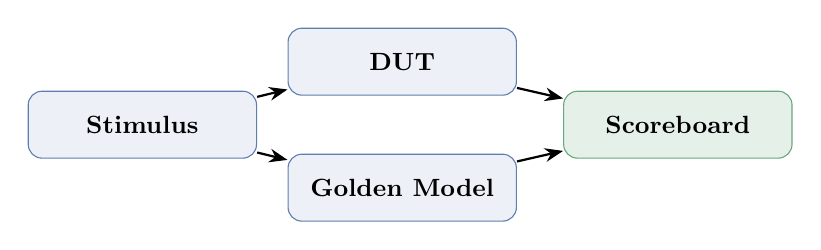
\begin{tikzpicture}[
        block/.style={draw=janusblue!70, fill=janusblue!8, rounded corners=5pt,
                      minimum width=2.9cm, minimum height=0.85cm,
                      align=center, font=\small\bfseries},
        arr/.style={-Stealth, thick}
      ]
        \node[block] (stim) at (0,1.3) {Stimulus};
        \node[block] (dut)  at (3.3,2.1) {DUT};
        \node[block] (gold) at (3.3,0.5) {Golden Model};
        \node[block, fill=verifygreen!12, draw=verifygreen!70] (score) at (6.8,1.3) {Scoreboard};
        \draw[arr] (stim) -- (dut);
        \draw[arr] (stim) -- (gold);
        \draw[arr] (dut) -- (score);
        \draw[arr] (gold) -- (score);
      \end{tikzpicture}
      \end{center}

      \vspace{0.6em}
      \begin{exampleblock}{CPU Example}
        After each retired instruction, compare the CPU's architectural state against Spike: PC, integer registers, and relevant memory locations.
      \end{exampleblock}
    \end{column}
  \end{columns}
\end{frame}

\begin{frame}{Assertions}
  \begin{columns}[T]
    \begin{column}{0.50\textwidth}
      An \textbf{assertion} is an executable statement of something that must always be true.

      \vspace{0.7em}
      \textbf{Why assertions help}
      \begin{itemize}
        \item catch bugs close to the source
        \item document design assumptions
        \item fail at the exact cycle of violation
        \item can be used in both simulation and formal verification
      \end{itemize}

      \vspace{0.7em}
      \textbf{Useful assertion targets in this lab}
      \begin{itemize}
        \item \texttt{x0} remains zero
        \item PC is word-aligned
        \item no write enable is asserted for a flushed instruction
        \item load-use hazard causes exactly one bubble
      \end{itemize}
    \end{column}
    \begin{column}{0.46\textwidth}
      \begin{block}{Immediate Assertion Style}
        Use ordinary Verilog checks in clocked blocks when SystemVerilog assertions are not available.
      \end{block}

      \vspace{0.6em}
      \begin{block}{Property Style}
        SystemVerilog Assertions (SVA) can express temporal rules such as ``if A happens this cycle, B must happen next cycle.''
      \end{block}

      \vspace{0.6em}
      \begin{alertblock}{Caution}
        An assertion is only as good as the rule it states. A wrong assertion can reject correct hardware or bless incorrect hardware.
      \end{alertblock}
    \end{column}
  \end{columns}
\end{frame}

\begin{frame}[fragile]{Assertion Examples for This CPU}
  \begin{columns}[T]
    \begin{column}{0.48\textwidth}
      \textbf{Immediate check in a testbench}
\begin{lstlisting}
always @(posedge clk) begin
  if (rst_n) begin
    if (u_cpu.u_reg_file.regs[0] !== 32'b0) begin
      $display("ASSERT FAIL: x0 changed");
      $finish;
    end
  end
end
\end{lstlisting}

      \vspace{0.4em}
      \small
      This catches any bug that writes a nonzero value into \texttt{x0}.
    \end{column}
    \begin{column}{0.48\textwidth}
      \textbf{SystemVerilog property style}
\begin{lstlisting}
property pc_word_aligned;
  @(posedge clk) disable iff (!rst_n)
    pc[1:0] == 2'b00;
endproperty

assert property (pc_word_aligned);
\end{lstlisting}

      \vspace{0.4em}
      \small
      If your tool or RTL subset does not support SVA, keep equivalent checks in the testbench.
    \end{column}
  \end{columns}
\end{frame}

\begin{frame}{Coverage: Did We Test Enough?}
  \begin{columns}[T]
    \begin{column}{0.48\textwidth}
      \textbf{Coverage} measures what your tests exercised.

      \vspace{0.7em}
      \textbf{Common coverage types}
      \begin{itemize}
        \item \textbf{Line coverage:} did each RTL line execute?
        \item \textbf{Branch coverage:} did each \texttt{if}/\texttt{case} path execute?
        \item \textbf{Toggle coverage:} did each signal bit change 0-to-1 and 1-to-0?
        \item \textbf{Functional coverage:} did meaningful scenarios happen?
      \end{itemize}
    \end{column}
    \begin{column}{0.48\textwidth}
      \begin{block}{CPU Functional Coverage Examples}
        \begin{itemize}\small
          \item every RV32I instruction executed at least once
          \item every immediate format used with positive and negative values
          \item every forwarding mux select value used
          \item load-use stall asserted and deasserted
          \item branch taken and not taken for every branch type
          \item writes to \texttt{x0} attempted
        \end{itemize}
      \end{block}

      \vspace{0.5em}
      \begin{alertblock}{Coverage Is Not Correctness}
        High coverage says a scenario happened. It does not automatically say the result was correct. Coverage needs checkers.
      \end{alertblock}
    \end{column}
  \end{columns}
\end{frame}

% =============================================================================
\section{CPU-Specific Verification}
% =============================================================================

\begin{frame}{What Is the CPU Contract?}
  \begin{columns}[T]
    \begin{column}{0.50\textwidth}
      The CPU has many internal wires, but software only sees the \textbf{architectural state}.

      \vspace{0.7em}
      \textbf{Architectural state for RV32I}
      \begin{itemize}
        \item \texttt{pc}: program counter
        \item \texttt{x0}--\texttt{x31}: integer registers
        \item data memory contents
        \item instruction memory contents as input program
      \end{itemize}

      \vspace{0.7em}
      A CPU implementation is correct if every retired instruction updates architectural state exactly as the ISA says.
    \end{column}
    \begin{column}{0.46\textwidth}
      \begin{block}{Microarchitecture Can Vary}
        A single-cycle CPU, a five-stage pipeline, and a superscalar CPU may have very different internal timing.
      \end{block}

      \vspace{0.6em}
      \begin{exampleblock}{But ISA Results Must Match}
        If the program executes:
        \texttt{addi x5, x0, 3}\\
        then after retirement, \texttt{x5} must be \texttt{3}, regardless of how many pipeline stages exist.
      \end{exampleblock}
    \end{column}
  \end{columns}
\end{frame}

\begin{frame}{Verification Levels for the Janus CPU}
  \begin{center}
  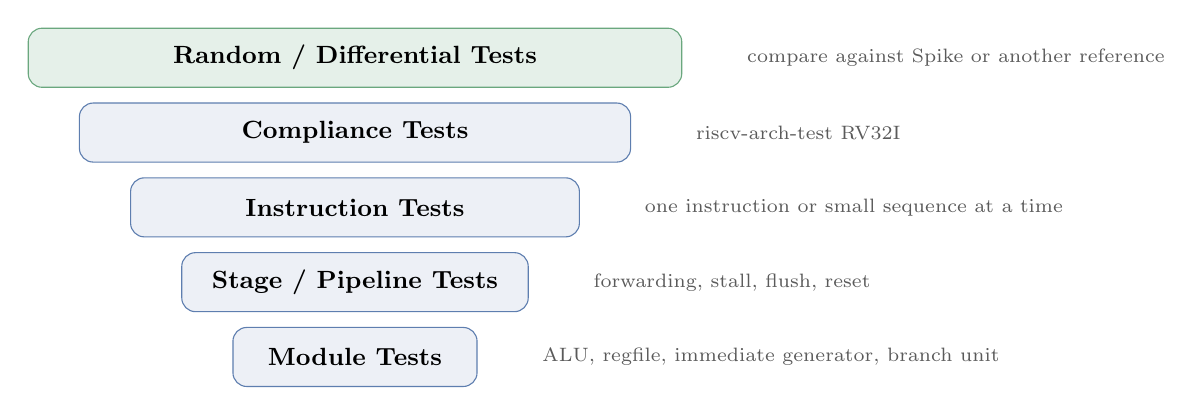
\begin{tikzpicture}[
    level/.style={draw=janusblue!70, fill=janusblue!8, rounded corners=5pt,
                  minimum width=#1, minimum height=0.75cm,
                  align=center, font=\small\bfseries},
    desc/.style={font=\scriptsize, align=center, text=janusgray}
  ]
    \node[level=3.1cm] (m) at (0,0) {Module Tests};
    \node[level=4.4cm] (s) at (0,0.95) {Stage / Pipeline Tests};
    \node[level=5.7cm] (i) at (0,1.90) {Instruction Tests};
    \node[level=7.0cm] (c) at (0,2.85) {Compliance Tests};
    \node[level=8.3cm, fill=verifygreen!12, draw=verifygreen!70] (r) at (0,3.80) {Random / Differential Tests};

    \node[desc, right=0.7cm of m] {ALU, regfile, immediate generator, branch unit};
    \node[desc, right=0.7cm of s] {forwarding, stall, flush, reset};
    \node[desc, right=0.7cm of i] {one instruction or small sequence at a time};
    \node[desc, right=0.7cm of c] {riscv-arch-test RV32I};
    \node[desc, right=0.7cm of r] {compare against Spike or another reference};
  \end{tikzpicture}
  \end{center}

  \vspace{0.5em}
  \small
  Work bottom-up during bring-up, then keep all levels in regression once the CPU starts executing programs.
\end{frame}

\begin{frame}{Module-Level Verification Examples}
  \renewcommand{\arraystretch}{1.2}
  \small
  \begin{tabular}{>{\bfseries\ttfamily}l p{4.5cm} p{5.8cm}}
    \toprule
    Module & What to Check & Important Corner Cases \\
    \midrule
    alu & every operation returns expected result and \texttt{zero} is correct & overflow wraparound, signed vs. unsigned compare, shift amount uses only low 5 bits \\
    \rowcolor{black!5}
    reg\_file & two async reads, one sync write, \texttt{x0} hardwired to zero & read-during-write, write \texttt{x0}, reset contents if required \\
    imm\_gen & immediate extraction and sign extension for I/S/B/U/J formats & negative branch offset, JAL bit scrambling, U-type low 12 bits zero \\
    \rowcolor{black!5}
    ctrl & opcode maps to correct control signals & invalid opcode becomes safe NOP, load/store enables not both high \\
    branch\_unit & every branch condition for signed and unsigned operands & \texttt{-1 < 1} signed, but \texttt{0xFFFF\_FFFF > 1} unsigned \\
    \rowcolor{black!5}
    dmem & byte/halfword/word load-store semantics & sign extension vs. zero extension, byte lanes, unaligned policy \\
    \bottomrule
  \end{tabular}
\end{frame}

\begin{frame}{Instruction-Level Test Matrix}
  \small
  \begin{columns}[T]
    \begin{column}{0.46\textwidth}
      \textbf{Arithmetic and logic}
      \begin{itemize}
        \item \texttt{ADD/SUB}: wraparound and negative operands
        \item \texttt{AND/OR/XOR}: alternating bit patterns
        \item \texttt{SLL/SRL/SRA}: shift by 0, 1, 31, and values with high bits set
        \item \texttt{SLT/SLTU}: same operands, different signedness
      \end{itemize}

      \vspace{0.6em}
      \textbf{Immediate instructions}
      \begin{itemize}
        \item smallest negative 12-bit immediate: \texttt{-2048}
        \item largest positive 12-bit immediate: \texttt{2047}
        \item \texttt{LUI}: lower 12 bits must be zero
        \item \texttt{AUIPC}: result depends on instruction PC
      \end{itemize}
    \end{column}
    \begin{column}{0.50\textwidth}
      \textbf{Memory}
      \begin{itemize}
        \item \texttt{LB/LH}: sign extension
        \item \texttt{LBU/LHU}: zero extension
        \item \texttt{SB/SH/SW}: byte-lane writes
        \item load after store to same address
      \end{itemize}

      \vspace{0.6em}
      \textbf{Control flow}
      \begin{itemize}
        \item all branch types taken and not taken
        \item forward branch and backward branch
        \item \texttt{JAL}: writes \texttt{pc+4} to \texttt{rd}
        \item \texttt{JALR}: target LSB is cleared
        \item branch or jump writing to \texttt{x0}
      \end{itemize}
    \end{column}
  \end{columns}
\end{frame}

\begin{frame}{Pipeline Hazard Verification}
  \begin{columns}[T]
    \begin{column}{0.50\textwidth}
      Pipeline verification checks whether the implementation preserves ISA behavior even when instructions overlap.

      \vspace{0.7em}
      \textbf{Hazards in this lab}
      \begin{itemize}
        \item \textbf{RAW}: read-after-write data dependency
        \item \textbf{Forwarding}: bypass EX/MEM or MEM/WB data into EX
        \item \textbf{Load-use}: one-cycle stall because load data is late
        \item \textbf{Control hazard}: taken branch/jump flushes wrong-path instructions
      \end{itemize}

      \vspace{0.6em}
      \begin{alertblock}{Key Debug Question}
        On the failing cycle, did the consumer instruction use the value from the register file, EX/MEM, MEM/WB, or memory?
      \end{alertblock}
    \end{column}
    \begin{column}{0.46\textwidth}
      \begin{block}{Signals to Inspect}
        \begin{itemize}\small
          \item \texttt{id\_rs1}, \texttt{id\_rs2}
          \item \texttt{ex\_rs1}, \texttt{ex\_rs2}, \texttt{ex\_rd}
          \item \texttt{mem\_rd}, \texttt{wb\_rd}
          \item \texttt{forward\_a}, \texttt{forward\_b}
          \item \texttt{pc\_stall}, \texttt{if\_id\_stall}
          \item \texttt{if\_id\_flush}, \texttt{id\_ex\_flush}
          \item \texttt{wb\_reg\_write}, \texttt{wb\_rd\_data}
        \end{itemize}
      \end{block}
    \end{column}
  \end{columns}
\end{frame}

\begin{frame}{Forwarding Timeline}
  \begin{center}
  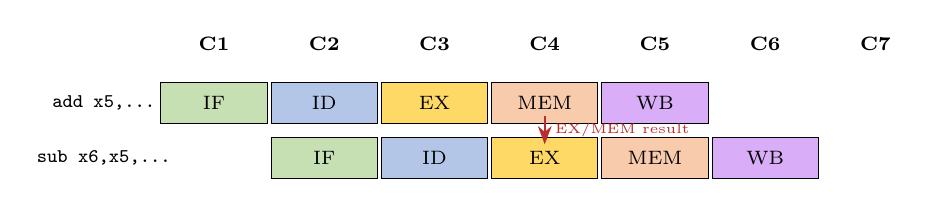
\begin{tikzpicture}[
    cell/.style={draw, minimum width=1.35cm, minimum height=0.52cm,
                 align=center, font=\scriptsize},
    hdr/.style={font=\scriptsize\bfseries},
    fwd/.style={-Stealth, thick, bugred}
  ]
    \foreach \i/\x in {1/1.4,2/2.8,3/4.2,4/5.6,5/7.0,6/8.4,7/9.8} {
      \node[hdr] at (\x,0.3) {C\i};
    }
    \node[hdr] at (0, -0.45) {\texttt{add x5,...}};
    \node[cell, fill=stageIF] at (1.4,-0.45) {IF};
    \node[cell, fill=stageID] at (2.8,-0.45) {ID};
    \node[cell, fill=stageEX] at (4.2,-0.45) {EX};
    \node[cell, fill=stageMEM] at (5.6,-0.45) {MEM};
    \node[cell, fill=stageWB] at (7.0,-0.45) {WB};

    \node[hdr] at (0, -1.15) {\texttt{sub x6,x5,...}};
    \node[cell, fill=stageIF] at (2.8,-1.15) {IF};
    \node[cell, fill=stageID] at (4.2,-1.15) {ID};
    \node[cell, fill=stageEX] at (5.6,-1.15) {EX};
    \node[cell, fill=stageMEM] at (7.0,-1.15) {MEM};
    \node[cell, fill=stageWB] at (8.4,-1.15) {WB};

    \draw[fwd] (5.6,-0.62) -- (5.6,-0.98)
      node[midway, right, font=\tiny, text=bugred] {EX/MEM result};
  \end{tikzpicture}
  \end{center}

  \vspace{0.6em}
  \begin{columns}[T]
    \begin{column}{0.48\textwidth}
      Producer \texttt{add} computes \texttt{x5} in EX during C3. The consumer \texttt{sub} needs \texttt{x5} in EX during C4.
    \end{column}
    \begin{column}{0.48\textwidth}
      The register file does not yet contain the new value, so \texttt{forward\_a} or \texttt{forward\_b} must select EX/MEM.
    \end{column}
  \end{columns}
\end{frame}

\begin{frame}{Load-Use Stall Timeline}
  \begin{center}
  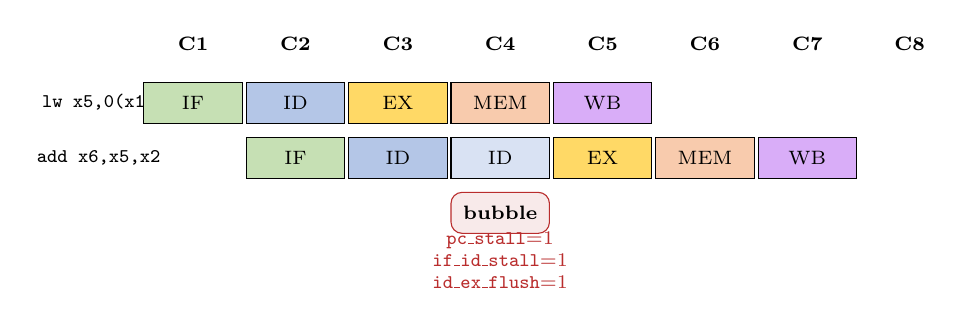
\begin{tikzpicture}[
    cell/.style={draw, minimum width=1.25cm, minimum height=0.52cm,
                 align=center, font=\scriptsize},
    hdr/.style={font=\scriptsize\bfseries},
    bubble/.style={draw=bugred, fill=bugred!10, rounded corners=4pt,
                   minimum width=1.25cm, minimum height=0.52cm,
                   align=center, font=\scriptsize\bfseries}
  ]
    \foreach \i/\x in {1/1.2,2/2.5,3/3.8,4/5.1,5/6.4,6/7.7,7/9.0,8/10.3} {
      \node[hdr] at (\x,0.3) {C\i};
    }
    \node[hdr] at (0, -0.45) {\texttt{lw x5,0(x1)}};
    \node[cell, fill=stageIF] at (1.2,-0.45) {IF};
    \node[cell, fill=stageID] at (2.5,-0.45) {ID};
    \node[cell, fill=stageEX] at (3.8,-0.45) {EX};
    \node[cell, fill=stageMEM] at (5.1,-0.45) {MEM};
    \node[cell, fill=stageWB] at (6.4,-0.45) {WB};

    \node[hdr] at (0, -1.15) {\texttt{add x6,x5,x2}};
    \node[cell, fill=stageIF] at (2.5,-1.15) {IF};
    \node[cell, fill=stageID] at (3.8,-1.15) {ID};
    \node[cell, fill=stageID!50] at (5.1,-1.15) {ID};
    \node[cell, fill=stageEX] at (6.4,-1.15) {EX};
    \node[cell, fill=stageMEM] at (7.7,-1.15) {MEM};
    \node[cell, fill=stageWB] at (9.0,-1.15) {WB};

    \node[bubble] at (5.1,-1.85) {bubble};
    \node[font=\scriptsize, text=bugred, align=center] at (5.1,-2.45)
      {\texttt{pc\_stall}=1\\\texttt{if\_id\_stall}=1\\\texttt{id\_ex\_flush}=1};
  \end{tikzpicture}
  \end{center}

  \vspace{0.4em}
  \small
  A load result is available after MEM, too late for the immediately following EX stage. One bubble gives the data time to reach MEM/WB for forwarding.
\end{frame}

\begin{frame}{Branch and Jump Flush Tests}
  \begin{columns}[T]
    \begin{column}{0.48\textwidth}
      A predict-not-taken pipeline fetches sequential instructions before it knows whether a branch is taken.

      \vspace{0.6em}
      \textbf{When a branch/jump resolves taken:}
      \begin{itemize}
        \item redirect PC to target
        \item flush wrong-path instruction in IF/ID
        \item flush wrong-path instruction in ID/EX
        \item ensure wrong-path register/memory writes do not happen
      \end{itemize}

      \vspace{0.6em}
      \begin{alertblock}{Most Important Check}
        Put a visible write on the wrong path. If the write commits, flush is broken.
      \end{alertblock}
    \end{column}
    \begin{column}{0.48\textwidth}
      \begin{block}{Directed Test Idea}
        \ttfamily\scriptsize
        addi x1, x0, 1\\
        beq  x1, x1, target\\
        addi x10, x0, 99 \quad // wrong path\\
        addi x11, x0, 99 \quad // wrong path\\
        target:\\
        bne  x10, x0, fail\\
        bne  x11, x0, fail\\
        pass
      \end{block}

      \vspace{0.6em}
      \begin{exampleblock}{Waveform Signals}
        Inspect \texttt{mem\_branch\_taken}, \texttt{mem\_jump}, \texttt{if\_id\_flush}, \texttt{id\_ex\_flush}, \texttt{wb\_rd}, and \texttt{wb\_reg\_write}.
      \end{exampleblock}
    \end{column}
  \end{columns}
\end{frame}

\begin{frame}{Memory Verification}
  \begin{columns}[T]
    \begin{column}{0.48\textwidth}
      Memory bugs are easy to miss because a simple demo often uses only \texttt{LW} and \texttt{SW}.

      \vspace{0.7em}
      \textbf{Load behavior}
      \begin{itemize}
        \item \texttt{LB}: load byte and sign-extend bit 7
        \item \texttt{LBU}: load byte and zero-extend
        \item \texttt{LH}: load halfword and sign-extend bit 15
        \item \texttt{LHU}: load halfword and zero-extend
        \item \texttt{LW}: load 32-bit word
      \end{itemize}
    \end{column}
    \begin{column}{0.48\textwidth}
      \textbf{Store behavior}
      \begin{itemize}
        \item \texttt{SB}: only one byte lane changes
        \item \texttt{SH}: only two byte lanes change
        \item \texttt{SW}: all four byte lanes change
        \item endianness matters: RISC-V is little-endian
      \end{itemize}

      \vspace{0.7em}
      \begin{block}{Lab Policy}
        The specification recommends word-aligned accesses. If your design rejects or ignores unaligned access, document the policy and test the aligned cases thoroughly.
      \end{block}
    \end{column}
  \end{columns}
\end{frame}

\begin{frame}{Differential Testing with an ISA Simulator}
  \begin{columns}[T]
    \begin{column}{0.50\textwidth}
      \textbf{Differential testing} runs the same program on two implementations and compares their behavior.

      \vspace{0.7em}
      For a RISC-V CPU:
      \begin{itemize}
        \item DUT: your RTL CPU in Verilator
        \item reference: Spike or another RISC-V ISA simulator
        \item compare architectural state after each retired instruction or at test end
      \end{itemize}

      \vspace{0.7em}
      \textbf{Why it is powerful}
      \begin{itemize}
        \item expected values do not need to be hand-written
        \item random programs become useful
        \item catches interactions between instructions
      \end{itemize}
    \end{column}
    \begin{column}{0.46\textwidth}
      \begin{block}{What Must Be Defined}
        \begin{itemize}\small
          \item When does an instruction retire?
          \item Which register writes count?
          \item Which memory writes count?
          \item How are traps, unsupported instructions, and timeouts handled?
        \end{itemize}
      \end{block}

      \vspace{0.7em}
      \begin{alertblock}{Beginner Scope}
        For this lab, start with end-of-test comparison and directed tests. Per-instruction differential testing is a good stretch goal.
      \end{alertblock}
    \end{column}
  \end{columns}
\end{frame}

\begin{frame}{RISC-V Architectural Tests}
  \begin{columns}[T]
    \begin{column}{0.48\textwidth}
      \texttt{riscv-arch-test} is a compliance-style test suite for RISC-V architectural behavior.

      \vspace{0.7em}
      \textbf{What it helps check}
      \begin{itemize}
        \item instruction semantics
        \item edge-case operands
        \item architectural register results
        \item ISA-level behavior independent of your microarchitecture
      \end{itemize}

      \vspace{0.7em}
      \textbf{Why after Phase 2?}
      \begin{itemize}
        \item pipeline hazards can corrupt otherwise-correct instruction logic
        \item compliance tests are more useful once basic execution is stable
      \end{itemize}
    \end{column}
    \begin{column}{0.48\textwidth}
      \begin{block}{What It Does Not Replace}
        \begin{itemize}\small
          \item module-level tests
          \item waveform debugging
          \item pipeline hazard directed tests
          \item memory-system tests specific to this lab
          \item assertions for internal invariants
        \end{itemize}
      \end{block}

      \vspace{0.7em}
      \begin{exampleblock}{Practical Use}
        Treat architectural tests as a regression milestone, not as your first debugging tool.
      \end{exampleblock}
    \end{column}
  \end{columns}
\end{frame}

% =============================================================================
\section{Static and Formal Checks}
% =============================================================================

\begin{frame}{Linting and Synthesis Sanity Checks}
  \begin{columns}[T]
    \begin{column}{0.50\textwidth}
      A simulator only explores the behavior your test drives. Static tools inspect the RTL structure.

      \vspace{0.7em}
      \textbf{Lint can catch}
      \begin{itemize}
        \item width mismatches
        \item unused signals
        \item implicit wires from typos
        \item incomplete combinational assignments
        \item suspicious blocking/nonblocking usage
      \end{itemize}

      \vspace{0.7em}
      \textbf{Synthesis check can catch}
      \begin{itemize}
        \item non-synthesizable constructs in RTL
        \item multiple drivers
        \item combinational loops
        \item unintended latches
      \end{itemize}
    \end{column}
    \begin{column}{0.46\textwidth}
      \begin{block}{Beginner Rule}
        Warnings are not decorations. Either fix them or write down why they are harmless.
      \end{block}

      \vspace{0.7em}
      \begin{exampleblock}{Tool Roles}
        \begin{itemize}\small
          \item \texttt{verilator --lint-only}: fast RTL lint
          \item \texttt{yosys check}: structural sanity after elaboration
          \item \texttt{verible-verilog-lint}: style and SystemVerilog lint where available
        \end{itemize}
      \end{exampleblock}
    \end{column}
  \end{columns}
\end{frame}

\begin{frame}[fragile]{Yosys Check Example}
  \begin{columns}[T]
    \begin{column}{0.48\textwidth}
      Yosys is primarily a synthesis tool, but it is also useful for sanity checking RTL.

      \vspace{0.7em}
      \textbf{Basic flow}
      \begin{enumerate}
        \item read Verilog
        \item choose top module
        \item convert processes
        \item optimize simple logic
        \item run structural checks
      \end{enumerate}

      \vspace{0.7em}
      This does not prove the CPU is correct, but it catches design hygiene problems before deeper tests.
    \end{column}
    \begin{column}{0.48\textwidth}
\begin{lstlisting}[language=Shell]
cd /foss/designs/janus_lab/cpu

yosys -p '
  read_verilog cpu.v
  hierarchy -top cpu
  proc
  opt
  check
'
\end{lstlisting}

      \vspace{0.4em}
      \begin{alertblock}{Testbench Exclusion}
        Do not synthesize \texttt{tb\_top.v}. Testbenches use simulation-only constructs such as \texttt{initial}, delays, \texttt{\$display}, and \texttt{\$dumpvars}.
      \end{alertblock}
    \end{column}
  \end{columns}
\end{frame}

\begin{frame}{Formal Verification: The Idea}
  \begin{columns}[T]
    \begin{column}{0.50\textwidth}
      Simulation asks:
      \begin{center}
        \large\textbf{``Does this behavior work for the tests I ran?''}
      \end{center}

      Formal verification asks:
      \begin{center}
        \large\textbf{``Can any legal behavior violate this property?''}
      \end{center}

      \vspace{0.7em}
      A formal tool explores many possible input combinations automatically, using mathematical solving instead of running one explicit test at a time.
    \end{column}
    \begin{column}{0.46\textwidth}
      \begin{block}{Good Formal Targets}
        \begin{itemize}\small
          \item small modules with clear contracts
          \item ALU properties
          \item register file \texttt{x0} invariant
          \item forwarding unit priority
          \item hazard unit output rules
        \end{itemize}
      \end{block}

      \vspace{0.6em}
      \begin{alertblock}{Hard Formal Targets}
        A full pipelined CPU with memories and arbitrary programs is much harder. Start small.
      \end{alertblock}
    \end{column}
  \end{columns}
\end{frame}

\begin{frame}[fragile]{Formal Property Examples}
  \begin{columns}[T]
    \begin{column}{0.48\textwidth}
      \textbf{ALU identity}
\begin{lstlisting}
// For every input a, ADD with zero returns a.
always @(*) begin
  if (alu_ctrl == ALU_ADD && b == 32'b0)
    assert(result == a);
end
\end{lstlisting}

      \vspace{0.5em}
      \textbf{Forwarding priority}
\begin{lstlisting}
// EX/MEM must win over MEM/WB.
always @(*) begin
  if (mem_reg_write && wb_reg_write &&
      mem_rd == ex_rs1 && wb_rd == ex_rs1 &&
      ex_rs1 != 5'b0)
    assert(forward_a == 2'b10);
end
\end{lstlisting}
    \end{column}
    \begin{column}{0.48\textwidth}
      \textbf{Hazard unit rule}
\begin{lstlisting}
always @(*) begin
  if (ex_mem_read && ex_rd != 5'b0 &&
      (ex_rd == id_rs1 || ex_rd == id_rs2)) begin
    assert(pc_stall);
    assert(if_id_stall);
    assert(id_ex_flush);
  end
end
\end{lstlisting}

      \vspace{0.5em}
      \small
      These properties are local and understandable. They are much easier to debug than a full CPU proof.
    \end{column}
  \end{columns}
\end{frame}

% =============================================================================
\section{Debugging Workflow}
% =============================================================================

\begin{frame}{Debugging a Failing CPU Test}
  \begin{center}
  \begin{tikzpicture}[
    step/.style={draw=janusblue!70, fill=janusblue!8, rounded corners=5pt,
                 minimum width=2.55cm, minimum height=0.86cm,
                 align=center, font=\small\bfseries},
    arr/.style={-Stealth, thick, janusblue}
  ]
    \node[step] (repro) at (0,0) {Reproduce};
    \node[step] (min) at (3.0,0) {Minimize};
    \node[step] (wave) at (6.0,0) {Open Wave};
    \node[step] (first) at (9.0,0) {Find First\\Bad Cycle};
    \node[step] (fix) at (12.0,0) {Fix and\\Regress};
    \draw[arr] (repro) -- (min);
    \draw[arr] (min) -- (wave);
    \draw[arr] (wave) -- (first);
    \draw[arr] (first) -- (fix);
  \end{tikzpicture}
  \end{center}

  \vspace{0.9em}
  \begin{columns}[T]
    \begin{column}{0.48\textwidth}
      \textbf{Do}
      \begin{itemize}
        \item keep the failing program short
        \item record seed/tool version if random
        \item inspect PC and pipeline registers first
        \item compare expected vs. actual at each stage
        \item rerun all old tests after a fix
      \end{itemize}
    \end{column}
    \begin{column}{0.48\textwidth}
      \textbf{Avoid}
      \begin{itemize}
        \item changing many modules at once
        \item trusting a passing waveform without a checker
        \item ignoring warnings
        \item fixing symptoms without identifying the first wrong cycle
        \item assuming the test is correct without checking disassembly
      \end{itemize}
    \end{column}
  \end{columns}
\end{frame}

\begin{frame}{Waveform Reading Checklist}
  \begin{columns}[T]
    \begin{column}{0.48\textwidth}
      Start with the smallest signal set that explains architectural progress.

      \vspace{0.6em}
      \textbf{Top-level}
      \begin{itemize}
        \item \texttt{clk}, \texttt{rst\_n}
        \item \texttt{cycle\_count}
        \item \texttt{pc}, \texttt{next\_pc}
        \item fetched \texttt{if\_instr}
      \end{itemize}

      \vspace{0.5em}
      \textbf{Pipeline identity}
      \begin{itemize}
        \item \texttt{id\_instr}, \texttt{ex\_rd}, \texttt{mem\_rd}, \texttt{wb\_rd}
        \item valid/flush/stall signals
        \item writeback enable and data
      \end{itemize}
    \end{column}
    \begin{column}{0.48\textwidth}
      \textbf{Data path}
      \begin{itemize}
        \item \texttt{id\_rs1\_data}, \texttt{id\_rs2\_data}
        \item \texttt{ex\_rs1\_data}, \texttt{ex\_rs2\_fwd}
        \item \texttt{alu\_result}
        \item \texttt{dmem\_rd\_data}
        \item \texttt{wb\_rd\_data}
      \end{itemize}

      \vspace{0.5em}
      \textbf{Control}
      \begin{itemize}
        \item \texttt{reg\_write}, \texttt{mem\_read}, \texttt{mem\_write}
        \item \texttt{branch}, \texttt{jump}, \texttt{branch\_taken}
        \item \texttt{forward\_a}, \texttt{forward\_b}
      \end{itemize}
    \end{column}
  \end{columns}
\end{frame}

\begin{frame}{Common Failure Patterns in This Lab}
  \renewcommand{\arraystretch}{1.2}
  \small
  \begin{tabular}{>{\bfseries}p{3.2cm} p{4.4cm} p{4.6cm}}
    \toprule
    Symptom & Likely Cause & First Signals to Check \\
    \midrule
    PC jumps to unknown & reset missing, next-PC mux uses \texttt{X}, uninitialized branch target & \texttt{rst\_n}, \texttt{pc}, \texttt{next\_pc}, \texttt{branch\_taken} \\
    \rowcolor{black!5}
    One arithmetic test fails & ALU control decode or signedness bug & \texttt{alu\_op}, \texttt{funct3}, \texttt{funct7}, \texttt{alu\_ctrl\_out} \\
    Load-use sequence fails & stall not asserted or bubble not inserted & \texttt{ex\_mem\_read}, \texttt{ex\_rd}, \texttt{pc\_stall}, \texttt{id\_ex\_flush} \\
    \rowcolor{black!5}
    Back-to-back ALU ops fail & forwarding select wrong or priority reversed & \texttt{forward\_a}, \texttt{forward\_b}, \texttt{mem\_rd}, \texttt{wb\_rd} \\
    Taken branch corrupts register & wrong-path instruction not flushed & \texttt{if\_id\_flush}, \texttt{id\_ex\_flush}, \texttt{wb\_reg\_write} \\
    \rowcolor{black!5}
    Byte loads wrong & sign/zero extension or endian bug & \texttt{funct3}, \texttt{addr[1:0]}, \texttt{rd\_data} \\
    \bottomrule
  \end{tabular}
\end{frame}

% =============================================================================
\section{Lab 02 Workflow}
% =============================================================================

\begin{frame}{Lab 02: Verify Your Own Lab 01 CPU}
  \begin{columns}[T]
    \begin{column}{0.50\textwidth}
      \textbf{Objective}\\
      Use the IIC-OSIC-TOOLS container to verify the CPU design you built in the first lab.

      \vspace{0.7em}
      \textbf{Required evidence}
      \begin{itemize}
        \item lint/smoke-test output
        \item at least five module-level tests
        \item at least ten instruction-level tests
        \item at least three hazard tests if your CPU is pipelined
        \item waveform screenshot or saved signal list for one debug case
        \item short report explaining bugs found and fixed
      \end{itemize}
    \end{column}
    \begin{column}{0.46\textwidth}
      \begin{block}{Recommended Test Order}
        \begin{enumerate}\small
          \item reset and PC
          \item ALU, immediate generator, register file
          \item arithmetic and logical instructions
          \item loads and stores
          \item branches and jumps
          \item forwarding, load-use, branch flush
          \item architectural regression suite
        \end{enumerate}
      \end{block}

      \vspace{0.6em}
      \begin{alertblock}{Deliverable Principle}
        A passing demo is not enough. Submit tests and evidence that explain what behavior was verified.
      \end{alertblock}
    \end{column}
  \end{columns}
\end{frame}

\begin{frame}[fragile]{A Practical Regression Script}
  \begin{columns}[T]
    \begin{column}{0.48\textwidth}
      A regression script runs tests repeatedly and consistently.

      \vspace{0.7em}
      Start simple:
      \begin{itemize}
        \item one command to lint
        \item one command per assembly test
        \item stop on the first failure
        \item print a summary
      \end{itemize}

      \vspace{0.7em}
      Later, add random seeds, coverage collection, and CI.
    \end{column}
    \begin{column}{0.48\textwidth}
\begin{lstlisting}[language=Shell]
#!/usr/bin/env bash
set -e

cd /foss/designs/janus_lab/cpu

verilator --lint-only -Wall -I. tb_top.v cpu.v

for t in tests/*.s; do
  echo "RUN $t"
  riscv64-unknown-elf-as \
    -march=rv32i -mabi=ilp32 \
    -o test.o "$t"
  riscv64-unknown-elf-ld \
    -Ttext=0x0 -o test.elf test.o
  riscv64-unknown-elf-objcopy \
    -O verilog test.elf program.hex
  verilator --binary -j 0 -I. tb_top.v cpu.v
  ./obj_dir/Vtb_top
done
\end{lstlisting}
    \end{column}
  \end{columns}
\end{frame}

\begin{frame}{What to Put in the Verification Report}
  \begin{columns}[T]
    \begin{column}{0.48\textwidth}
      \textbf{Environment}
      \begin{itemize}
        \item IIC-OSIC-TOOLS image tag
        \item simulator versions
        \item command lines used
      \end{itemize}

      \vspace{0.6em}
      \textbf{Test Plan}
      \begin{itemize}
        \item features tested
        \item tests mapped to features
        \item expected results and checkers
      \end{itemize}

      \vspace{0.6em}
      \textbf{Results}
      \begin{itemize}
        \item pass/fail table
        \item bug list
        \item remaining known limitations
      \end{itemize}
    \end{column}
    \begin{column}{0.48\textwidth}
      \begin{block}{Bug Report Template}
        \renewcommand{\arraystretch}{1.15}
        \scriptsize
        \begin{tabular}{p{2.3cm}p{4.2cm}}
          \toprule
          Field & Content \\
          \midrule
          Symptom & What failed? \\
          Test & Which test exposed it? \\
          Root cause & Which RTL rule was wrong? \\
          Fix & What changed? \\
          Evidence & Which regression now passes? \\
          \bottomrule
        \end{tabular}
      \end{block}

      \vspace{0.7em}
      \begin{exampleblock}{Good Engineering Habit}
        When you fix a bug, keep the test that found it. That test becomes part of the regression suite.
      \end{exampleblock}
    \end{column}
  \end{columns}
\end{frame}

% =============================================================================
\section{Summary}
% =============================================================================

\begin{frame}{Key Takeaways}
  \begin{columns}[T]
    \begin{column}{0.48\textwidth}
      \textbf{Verification basics}
      \begin{itemize}
        \item verification collects evidence against a specification
        \item testbenches drive, observe, and check the DUT
        \item self-checking tests are required for regression
        \item waveforms are for debugging, not the final proof of pass/fail
        \item warnings from lint/synthesis tools deserve attention
      \end{itemize}

      \vspace{0.6em}
      \textbf{Toolflow}
      \begin{itemize}
        \item Verilator/Icarus: RTL simulation
        \item GTKWave: waveform inspection
        \item Yosys: synthesis and structural checks
        \item Spike: RISC-V ISA reference
      \end{itemize}
    \end{column}
    \begin{column}{0.48\textwidth}
      \textbf{CPU-specific verification}
      \begin{itemize}
        \item architectural state is the CPU contract
        \item module tests isolate bugs early
        \item instruction tests check ISA behavior
        \item hazard tests check pipeline timing
        \item assertions document invariants
        \item coverage tells you what scenarios were exercised
      \end{itemize}

      \vspace{0.6em}
      \textbf{Debug discipline}
      \begin{itemize}
        \item reproduce, minimize, inspect, fix, regress
        \item identify the first wrong cycle
        \item keep every bug-finding test
      \end{itemize}
    \end{column}
  \end{columns}
\end{frame}

\begin{frame}{References and Starting Points}
  \begin{columns}[T]
    \begin{column}{0.48\textwidth}
      \textbf{Local lab files}
      \begin{itemize}
        \item \texttt{docs/spec.md}: CPU and lab specification
        \item \texttt{cpu/tb\_top.v}: top-level simulation testbench
        \item \texttt{cpu/cpu.v}: pipelined CPU top-level
        \item \texttt{cpu/hazard\_unit.v}: stall and flush control
        \item \texttt{cpu/forward\_unit.v}: operand forwarding control
      \end{itemize}
    \end{column}
    \begin{column}{0.48\textwidth}
      \textbf{Tool references}
      \begin{itemize}
        \item IIC-OSIC-TOOLS: \texttt{github.com/iic-jku/IIC-OSIC-TOOLS}
        \item Verilator: \texttt{verilator.org}
        \item Yosys: \texttt{yosyshq.net/yosys}
        \item GTKWave: \texttt{gtkwave.sourceforge.net}
        \item RISC-V architectural tests: \texttt{github.com/riscv-non-isa/riscv-arch-test}
      \end{itemize}

      \vspace{0.6em}
      \begin{exampleblock}{Next Lab}
        Bring your Lab 01 CPU into the container, run smoke tests, add self-checking tests, and produce a verification report.
      \end{exampleblock}
    \end{column}
  \end{columns}
\end{frame}

% -- Final slide ---------------------------------------------------------------
\begin{frame}
  \begin{center}
    \vspace{1.5em}
    {\Large\textbf{Questions?}}\\[1.5em]
    \large Janus Lab --- CPU Design and Implementation\\[0.5em]
    \normalsize Lecture 02: Hardware and CPU Verification\\[2em]
    \small
    \begin{tabular}{ll}
      Spec:      & \texttt{docs/spec.md} \\
      CPU RTL:   & \texttt{cpu/*.v} \\
      Testbench: & \texttt{cpu/tb\_top.v} \\
      Tools:     & \texttt{Verilator, GTKWave, Yosys, Spike} \\
    \end{tabular}
  \end{center}
\end{frame}

\end{document}
